\documentclass[a4paper, 11pt]{book}

\newcommand*{\plogo}{\fbox{$\mathcal{DB}$}}

\usepackage[utf8]{inputenc}
\usepackage{stix}
\usepackage[english]{babel}
\usepackage{amsfonts}
\usepackage{amsthm}
\usepackage{amsmath}
\usepackage{amssymb}
\usepackage{nicefrac}
\usepackage{commath}
\usepackage{dirtytalk}

\usepackage{graphicx}

\newtheorem{theorem}{Theorem}
\newtheorem{es}{Examples}
\newtheorem*{example}{Example}
\newtheorem{obs}{Observation}

\newcommand\restr[2]{{% we make the whole thing an ordinary symbol
    \left.\kern-\nulldelimiterspace % automatically resize the bar with \right
    #1 % the function
    \vphantom{\big|} % pretend it's a little taller at normal size
    \right|_{#2} % this is the delimiter
}}

\theoremstyle{definition}
\newtheorem{definition}{Definition}[section]
 
\theoremstyle{remark}
\newtheorem*{remark}{Remark}

\newtheorem{corollary}{Corollary}[theorem]
\newtheorem{lemma}[theorem]{Lemma}

\newtheorem{prop}{Proposition}

\newcommand{\inter}[1]{int(#1)}

\begin{document}

    \begin{titlepage} 
        \raggedleft

        \rule{1pt}{\textheight} % Vertical line
        \hspace{0.05\textwidth} % Whitespace between the vertical line and title page text
        \parbox[b]{0.75\textwidth}{ % Paragraph box for holding the title page text, adjust the width to move the title page 
            % left or right on the page
                            
            {\Huge\bfseries MATC37 Lecture \\[0.5\baselineskip] Notes }\\[2\baselineskip] % Title
            {\large\textit{Lecture notes on a course in real analysis}}\\[4\baselineskip] % Subtitle or further description
            {\Large\textsc{A. Wortschöpfer}} % Author name, lower case for consistent small caps
                                                    
            \vspace{0.5\textheight} % Whitespace between the title block and the publisher
                                                            
            {\noindent The Publisher~~\plogo}\\[\baselineskip] % Publisher and logo
        }
    \end{titlepage}

    \chapter{Shortcomings of the Riemann integral}

    In the turn of the 19th century many mathematicians were starting to discover that the Riemann integral had many shortcomings
    and were starting to look for a new formulation. Thus, was born the Lebesgue integral. Here we will discuss some of the problems
    that motivated the idea for the Lebesgue measure and the Lebesgue integral.

    \section{Limits of continuous functions}

    Let $f: [0,1] \to \mathbb{R}$ be continuous. Let $f_n: [0,1] \to \mathbb{R}$ be a continuous function so that
    $\{f_n\}_{n\in\mathbb{N}}$ is a sequence of continuous functions on the interval $[0,1]$. Assume that
    \[ \lim_{n\to\infty} f_n(x) = f(x) \]
    exists for every $x\in[0,1]$. We know from MATB43 that if each $f_n$ is uniformily continuous, then $f$ is continuous but suppose
    each $f_n$ were not uniformily continuous, then there are issues that may arise which may seem subtle but have radical effects.
    For example, we can construct a sequence of continuous functions $\{f_n\}$ converging everywhere to $f$ so that
    \begin{enumerate}
        \item[(a)] $0\leq f_n(x)\leq 1$ for all $x$
        \item[(b)] $f_n \geq f_{n+1}$ i.e. the sequence $\{f_n\}$ is monotonically decreasing as $n\to\infty$.
        \item[(c)] $f(x) = \lim_{n\to\infty} f_n(x)$ exists for all $x$
    \end{enumerate}
    However, $f$ is not Riemann integrable!\\
    Note that, in view of (b), we obtain $\int_0^1 f_n(x)dx \geq \int_0^1 f_{n+1}(x)dx$. Combining this with the fact that there is
    a lower bound (using (a)) on $\int_0^1 f_n(x)dx$, we know that the sequence $\int_0^1 f_n(x)dx$ converges to a limit.
    Therefore, the question arises: What method of integration can be used to integrate $f$ and obtain that for it
    \[ \int_0^1 \lim_{n\to\infty} f_n(x)dx = \lim_{n\to\infty} \int_0^1 f_n(x)dx \]
    It is with Lebesgue integration that we can solve this problem.

    \section{Irregular Geometric Objects}
    We say a curve is \textbf{rectifiable} if its length $L$ (defined in terms of the supremum of lengths of all polygonal lines
    joining successively finitely many points of the curve) is finite. Rectifiable curves, because they are endowed with length are
    one-dimensional in nature. However, it is worth asking if there are non-rectifiable curves which are two-dimensional or rather just
    any dimensions more than one. We shall see the answer to this question in terms of space-filling curves and generally have dimensions
    between 1 and 2.\\
    Recall our area/length definitions for regular polygons. It is worth asking if we can extend our understanding of area and length
    so that we can measure geometric objects that are not as simple as regular polygons such as fractional objects such as
    Koch's snowflake. Note these objects are still parameterized by lines so this question and the previous are well connected.

    \section{Differentiation and Integration}
    The fundamental theorem of calculus expresses the notion that differentiation and integration are inverse operations and it
    does this via the two equations below
    \begin{align}
        F(b) - F(a) &= \int_a^b F'(x)dx, \\
        \nicefrac{d}{dx}\int_0^x f(y)dy &= f(x).
    \end{align}
    It is natural to try and find a general class of functions which respect either of these equations. However, for the first
    equation, the existence of continuous functions $F$ which are nowhere differentiable, or for which $F'(x)$ exists for every
    $x$, but $F'$ is not integrable, leads to the problm of finding a general class of functions for which this equation is valid.
    For the second equation, the question is to formulate properly and establish this assertion for the general class of integrable
    functions $f$. These questions can be answered with the help of certain covering arguments, and the notion of absolute continuity.

    \section{Probability Theory}
    Define $S$ to be a space of $\{0,1\}$-valued sequences (e.g. fair coin toss). Define $f: S \to [0,1]$ where
    \[ f(s) = \sum_{n=1}^{\infty} \nicefrac{S_n}{2^n} \]
    Note this implies $0\leq f \leq 1$.
    Then, we can compute,
    \[ P(s_1=0,s_2=1) = l([\nicefrac{1}{4},\nicefrac{1}{2}]) = \nicefrac{1}{4} \]
    However, what happens if we try to take an arbitrary set $A\subset [0,1]$ and try to compute $P(f^{-1}(A)) = l(A)$. This problem
    is answered (not completely, however) by the Lebesgue measure.

    \section{The measure problem (MP)}

    To put matters clearly, the fundamental issue that must be understood in order to try to answer all of the questions raised above
    is that of measure. Stated impercisely in one dimension, we are trying to assign to each subset $E$ of $\mathbb{R}$ its 
    one-dimensional measure $l(E)$, that is, its length, thereby extending the standard notion of length defined for closed intervals.
    For example, consider the sets below:
    \[ (i)\: [2,6] \quad (ii)\: (2,6] \quad (iii)\: \{2\} \quad (iv)\: \mathbb{R} \quad (v)\: \mathbb{Q} \quad (vi) 
        \cup_{n=1}^{\infty} [n,n+\nicefrac{1}{n^2}] \quad (vii)\: \emptyset\]
    It seems intuitive to assign 4 to (i) so that $l([2,6]) = 6 - 2 = 4$. We can assign (ii) the same measure as well. (iii) is just
    a single point so it is a 0 dimensional object, therefore it seems intuitive to assign it the measure 0 so that $l(\{2\}) = 0$.
    We assign (vii) the same measure since it contains \textit{no} points whatsoever. There is no intuitive way to assign
    $\mathbb{R}$ a finite measure, therefore we write $l(\mathbb{R}) = \infty$. However, we cannot apply the same reasoning to (v).
    Recall from MATB43 that any countable set has Lebesgue measure zero, therefore we write $l(\mathbb{Q}) = 0$. (vi) is a bit tricky
    but easily understood if we remember that $l([n,n+\nicefrac{1}{n^2}]) = (n+\nicefrac{1}{n^2}) - n = \nicefrac{1}{n^2}$ so that
    \[ l(\cup_{n} [n,n+\nicefrac{1}{n^2}]) = \sum_n l([n,n+\nicefrac{1}{n^2}]) = \sum_n \nicefrac{1}{n^2} = \nicefrac{\pi^2}{6} \]
    Moving from left-most part to the second-left most part is done through a equality that we have not yet proven but it does
    seem intuitive to want this to be true. Therefore, we should want $l$ to have this property.\\
    Before, we move on further, it is important to discuss the closely related integral problem as well.

    \subsection{The integral problem (IP)}
    This is concerned with the question: For which $f: [0,1]\to\mathbb{R}$ can we make sense of $\int_0^1 f(x)dx$? Thus, we are
    concerned with finding the class of integrable functions. Note that MP and IP are closely related.\\
    Given a set $A\subset\mathbb{R}$, consider the characteristic function
    \[ \mathcal{X}(A) = \begin{cases} 
            1, & x\in A \\
            0  & x\not\in A
       \end{cases} \]
   Then $\int \mathcal{X}_A(x)dx = l(A)$ i.e. integrating the characteristic function over a set is the same as taking its measure.\\
   Conversely, given $f:[0,1]\to\mathbb{R}$ we can try to write $f$ as 
   \[ f = \sum_n a_n\mathcal{X}_{A_n} \]
   for some suitable $a_n\in\mathbb{R}$ and $A_n\subset\mathbb{R}$ and then we try to compute
   \[ \int f(x)dx = \int \sum_n a_n\mathcal{X}_{A_n}dx = \sum a_n\int \mathcal{X}_{A_n}dx = \sum a_nl(A_n) \]
   Note, we actually used the equality mentioned in section 1.1.

   \section{Wishlist for MP}
   We are looking for a non-negative (length intuitively should be non-negative) function $m$ defined on any given subset of 
   $\mathbb{R}$. Therefore, we are looking for a function $l: \mathcal{P}(\mathbb{R}) \to \mathbb{R}^{+}$ such that:
   \begin{enumerate}
       \item If $A_1,A_2,\hdots$ are disjoint then
           \[ l(\bigcup_{n} A_n) = \sum_n l(A_n) \]
           This is called the \textbf{countably additive} property.
       \item $l(A+t) = l(A)$ for any $t\in\mathbb{R}$. This is called the \textbf{translation invariance} property.
       \item $l([0,1]) = 1$ i.e. $l$ is \textit{normalized} 
   \end{enumerate}

   However, we shall see that this is an unrealistic wishlist.

   \begin{theorem}[Vitali, 1905]
       There does not exist a measure $l: \mathcal{P}(\mathbb{R}) \to [0,\infty]$ such it satisfies all the properties above.
   \end{theorem}
   \begin{proof}
       Define an equivalence relation on the closed unit interval $\mathbb{I} = [0,1]$ via
       \[ \forall\;x,y\in\mathbb{I}:\;x\sim y \Leftrightarrow x-y\in\mathbb{Q} \]
       Then, we have a natural set of elements of each equivalence class given by $\sim$. Denote this set by $A$. Note,
       $M\subset\mathbb{I}$ and for each $x\in\mathbb{R}$ there exists a unique $y\in A$ and $r\in\mathbb{Q}$ such that
       $x = y + r$.\\
       Then, define
       \[ A_r := \{y+r: y\in A\} \]
       for each $r\in\mathbb{Q}$. Because of what we noted above, we obtain the result that $\mathbb{R}$ is partitioned
       into countably many disjoint sets, and specifically by the sets:
       \[ \mathbb{R} := \bigcup \{A_r: r\in\mathbb{Q}\} \]
       Suppose that $A$ is measurable by $l$. Then:
       \[ 1 = l([0,1]) = \sum_{r\in\mathbb{Q}} l(A_r) = l(A) \]
       Then $l(A)\neq 0$ since by countable additivity, we would have $l([0,1]) = 0$. Suppose $l(A)>0$. Then
       \begin{align*}
           l([0,1]) \geq l(\bigcup_{r\in\mathbb{Q}\cap[0,1]} A_r) = \sum_{r\in\mathbb{Q}\cap[0,1]} l(A_r) = \infty
       \end{align*}
       since $l(A_r) = l(A)$ by translation invariance. But this is also a contradiction as $1 \geq \infty$. Therefore,
       $l$ cannot satisfy \textit{every} property above.
   \end{proof}

   It is because of this that we loosen our wishlist to allow the existence of non-measurable sets. The reader is warned
   that constructions of such sets are not trivial!\\

   If we try to loosen countable additivity to just \textit{finite} additivity, it is still too strong. Consider the Banach-Tarski
   paradox (very non trivial to prove so it will not be done here). This is possible by assuming all properties above but replacing
   countable additivity by finite additivity. It turns out that such a measure can exist in $\mathbb{R}^1$ but not any higher.

   \begin{theorem}[Banach-Tarski Paradox]
       The three-dimensional unit ball can be decomposed into a finite number of disjoint sets, which can then be reassembelled
       into two three-dimensional unit balls.
   \end{theorem}

    While this is not a contradiction but it does allow for highly non intuitive results.

    \chapter{Measure Theory}

    \section{Preliminaries}

    This section is devoted to reviewing the basic notions that one has in $\mathbb{R}^d$ (positive integer $d$).\\

    The rational numbers are denoted by $\mathbb{Q}$. The real numbers are denoted by $\mathbb{R}$ and can be written as
    $(-\infty,+\infty)$. The extended real numbers are written as $\mathbb{R}\cup\{\pm \infty\}$ or $[-\infty,+\infty]$.\\

    \begin{definition}
        Fix an integer $d\geq 1$. A \textbf{point} $x\in\mathbb{R}^d$ is given by an ordered $d$-tuple of real numbers 
        ($\mathbb{R}^1$),
        \[ \mathbf{x} = (x_1,\hdots,x_d)\qquad\text{where}\qquad x_1,\hdots,x_d\in\mathbb{R} \]
        $\mathbb{R}^d$ is called the \textbf{$d$-dimensional Euclidean space}.
    \end{definition}

    Recall, that we can add vectors (points in a Euclidean space),
    \[ \mathbf{x} = (x_1,\hdots,x_d),\;\mathbf{y} = (y_1,\hdots,y_d)\implies \mathbf{x}+\mathbf{y} = (x_1+y_1,\hdots,x_d+y_d) \]
    and multiply them by a scalar $\lambda\in\mathbb{R}$,
    \[ \lambda\mathbf{x} = (\lambda x_1,\hdots,\lambda x_d) \]

    \begin{definition}
        The \textbf{norm} of $x\in\mathbb{R}^d$ is defined as $|x| = (\sum x_i^2)^{\nicefrac{1}{2}}$. The norm operator has
        the following properties,
        \begin{itemize}
            \item $|x|\geq 0$ and $|x|=0$ if and only if $x=0$.
            \item $|\lambda x| = |\lambda||x|$
            \item $|x+y| \leq |x| + |y|$
        \end{itemize}
    \end{definition}

    In particular, we can \textit{measure} the distance between $x,y\in\mathbb{R}^d$ via
    \[ d(x,y) := |x-y| \]
    where $d$ is then a function $d:\mathbb{R}^d\times\mathbb{R}^d\to[0,\infty)$ most comonly called the \textbf{distance function}
    with the following properties:
    \begin{enumerate}
        \item $d(x,y)\geq 0$ and $d(x,y)=0$ if and only if $x=y$
        \item $d(x,y) = d(y,x)$
        \item $d(x,z) = d(x,y) + d(y,z)$ for $x,y,z\in \mathbb{R}^d$
    \end{enumerate}

    \begin{definition}
        For a set $E\subset\mathbb{R}^d$, the \textbf{complement} is
        \[ E^c := \{x\in\mathbb{R}^d: x\not\in E\} = \mathbb{R}^d\textbackslash E \]
        More generally, for two sets $E,F\subset\mathbb{R}^d$, we have the \textbf{difference of two sets} being given by
        \[ F\textbackslash E := \{x\in\mathbb{R}^d: x\in F\;\text{and}\;x\not\in E\} \]
        Also, recall
        \[ E \cup F = \{x\in\mathbb{R}^d: x\in E\;\text{and}\;x\in F\}\qquad(\textbf{union}) \]
        \[ E \cap F = \{x\in\mathbb{R}^d: x\in E\;\text{and}\;x\in F\}\qquad(\textbf{intersection}) \]

        Finally, for $E,F\subset\mathbb{R}^d$ define the \textbf{distance between sets} by
        \[ d(E,F) := \text{inf}_{x\in E, y\in F} d(x,y) \]
    \end{definition}

    This "$d$" is not to be confused with the one above because it does not have \textit{all} of the properties that the distance
    function between points does. Namely, if $E = (0,1)$ and $F = (1,2)$, then $d(E,F)=0$ but $E\neq F$, and in fact 
    $E\cap F=\emptyset$.

    \subsection{Open, Closed and Compact sets}

    \begin{definition}
        For $x\in\mathbb{R}^d$ and $r>0$, define
        \[ B_r(x) := \{y\in\mathbb{R}^d: d(x,y)<r\} \]
        $B_r(x)$ is said to be an \textbf{open ball} of radius $r$. A subset $E$ of $\mathbb{R}^d$ is \textbf{open} if for all $x\in E$,
        there exists $r>0$ such that $B_r(x)\subset E$.
    \end{definition}

    \begin{prop}
        An open ball $B_r(x)$ is open.
    \end{prop}
    \begin{proof}
        Given any point $\widetilde{x}\in B_r(x)$, we want to find $\widetilde{r}>0$ such that 
        $B_{\widetilde{r}}(\widetilde{x})\subset B_r(x)$.\\

        Set $\widetilde{r} = r - d(\widetilde{x},x)$. We know $\widetilde{r}$ is positive since $d(\widetilde{x},x)<r$ (definition
        of an open ball), which implies $\widetilde{r}>0$. Now if $z\in B_{\widetilde{r}}(\widetilde{x})$, then
        \[ d(x,z) \leq d(x,\widetilde{x}) + d(\widetilde{x},z) \leq d(x,\widetilde{x}) + \widetilde{r} = r\]
        Thus $z\in B_r(x)$. Hence $B_{\widetilde{r}}(\widetilde{x})\subset B_r(x)$ as wanted.
    \end{proof}

    \begin{prop}
        \begin{enumerate}
            \item $\emptyset$ and $\mathbb{R}^d$ are open.
            \item If $\{\theta_{\alpha}\}$ is a collection of open sets, then $\cup_{\alpha}\theta_{\alpha}$ is open.
            \item If $\theta_{\alpha_1},\hdots,\theta_{\alpha_n}$ are open, then $\cap_{i=1}^n \theta_{\alpha_i}$ is open.
        \end{enumerate}
    \end{prop}
    \begin{proof}
        \begin{enumerate}
            \item Clear.
            \item Choose $x\in\cup_{\alpha}\theta_{\alpha}$. Then there exists $\alpha'$ such that $x\in \theta_{\alpha'}$. Because
                $\theta_{\alpha'}$ is an open set, there exists a $r>0$ such that 
                $B_r(x)\subset\theta_{\alpha'}\subset\cup_{\alpha}\theta_{\alpha}$ as wanted.
            \item Let $x\in\cap_{i=1}^n \theta_{\alpha_i}$, then there exists $r_1,\hdots,r_n$ such that 
                $B_{r_1}(x)\subset\theta_{\alpha_1},\hdots,B_{r_n}(x)\subset\theta_{\alpha_n}$.
        \end{enumerate}
    \end{proof}

    \begin{remark}
        (3) only works for a finite collection. For example, $\cap_{n=1}^{\infty} (-\nicefrac{1}{n},\nicefrac{1}{n}) = \{0\}$ which
        is not open!
    \end{remark}

    \begin{definition}
        A set $E\subset \mathbb{R}^d$ is \textbf{closed} if $E^c$ is open.
    \end{definition}

    \begin{example}
        \begin{enumerate}
            \item $[0,1]\subset\mathbb{R}$ is closed. Indeed, $[0,1]^c = (-\infty, 0) \cup (1,\infty)$.
            \item $\emptyset$ and $\mathbb{R}^d$ are both open and closed.
        \end{enumerate}
    \end{example}

    Note that most sets are neither open nor closed e.g. $(0,1]\subset \mathbb{R}$ is not open or closed.

    \begin{definition}
        A set $E$ is \textbf{bounded} if it is contained in some ball of finite radius. A bounded set is \textbf{compact}
        if it is also closed. Compact sets can also be defined using the Heine-Borel property:\\
        If $E$ is covered by some collection $\{Q_{\alpha}\}$ of open sets (called an \textbf{open cover}), then there are
        finitely many of the open sets $Q_{\alpha_1},\hdots,Q_{\alpha_n}$ such that $E$ is also covered by this finite collection
        of open sets from $\{Q_{\alpha}\}$ (called a \textbf{finite subcover}).
    \end{definition}

    \begin{definition}
        A point $x\in\mathbb{R}^d$ is a \textbf{limit point} of the set $E$ is for every $r>0$, the ball $B_r(x)$ contains
        points of $E$. An \textbf{isolated point} of $E$ is a point $x\in E$ such that there exists an $r>0$ where
        $B_r(x)\cap E = \{x\}$.
    \end{definition}

    \begin{definition}
        A point $x\in E$ is an interior point of $E$ if there exists $r>0$ such that $B_r(x) \subset E$. The set of all interior
        points of $E$ is called the \textbf{interior} of $E$. Also, the \textbf{closure} $\overline{E}$ of $E$ consists of the
        union of $E$ and all of its limit points. The \textbf{boundary} of a set $E$, denoted by $\partial{E}$, is the set of
        points which are in the closure of $E$ but not in the interior of $E$. Note that the closure can be defined as the
        \textit{smallest} closed set which \textit{contains} $E$ and similarly, the interior of a set can be defined as the
        \textit{largest} open set which is \textit{contained in} $E$.
    \end{definition}

    \subsection{Rectangles and Cubes}

    \begin{definition}
        $R\subset\mathbb{R}^d$ is said to be a \textbf{closed rectangle} if it can be written in the form:
        \[ R = [a_1,b_1]\times\hdots\times [a_n,b_n] = \{(x_1,\hdots,x_n)\in\mathbb{R}^d: a_j\leq x\leq b_j, j=1,\hdots,n\} \]
        A \textbf{cube} is a rectangle for which $b_1-a_1=b_2-a_2=\hdots=b_d-a_d$.
    \end{definition}

    Note each rectangle $R$ has sides parallel to the coordinates axes and is closed.

    \begin{example}
        In $\mathbb{R}$, rectangles are line segments, in $\mathbb{R}^2$, rectangles are the usual 2-d flat, 4 sided polygons we
        see in high school and rectangles in $\mathbb{R}^3$ are called parallelepipeds.
    \end{example}

    \begin{definition}
        We say that the lengths of the sides of the rectangle $R$ are $b_1-a_1,\hdots,b_d-a_d$. The \textbf{volume} of the rectangle
        $R$ is denoted by $|R|$ and is defined to be
        \[ |R| = (b_1-a_1)\cdot\cdot\cdot(b_d-a_d) \]
    \end{definition}

    Continuing our most recent example, in $d=1$, the volume equals the length of the line segment and when $d=2$, it equals the area.

    \begin{definition}
        An open rectangle is the product of open intervals, and the interior of the rectangle $R$ is then
        \[ (a_1,b_1)\times(a_2,b_2)\times\cdot\cdot\cdot\times(a_d,b_d) \]
    \end{definition}

    \begin{definition}
        A union of rectangles is said to be \textbf{almost disjoint} if the interiors of the rectangles are disjoint.
    \end{definition}

    We shall make much use of coverings of sets with sets of rectangles and cubes. Some important results for these techniques
    is discussed:

    \begin{lemma}
        If a rectangle is the almost disjoint union of finitely many other rectangles, say $R = \cup_{k=1}^N R_k$, then
        \[ |R| = \sum_{k=1}^N |R_k| \]
    \end{lemma}

    \begin{proof}
        We consider the grid formed by extending indefinitely the sides of all rectangles $R_1,\hdots,R_N$. This construction yields
        finitely many rectangles $\hat{R_1},\hdots,\hat{R_M}$, and a partition $J_1,\hdots,J_N$ of the integers between 1 and $M$,
        such that the unions
        \[ R = \bigcup_{j=1}^M \hat{R_j}\quad\text{and}\quad R_k=\bigcup_{j\in J_k}\hat{R_j},\qquad\text{for}\:k=1,\hdots,N \]
        are almost disjoint.
        \begin{center}
            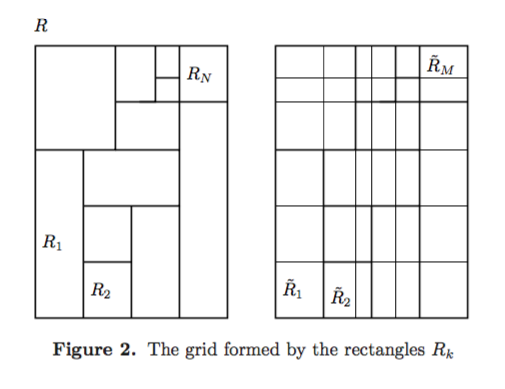
\includegraphics[scale=0.5]{fig2}\\
        \end{center}
        For the rectangle $R$, for example, we see that $|R| = \sum_{j=1}^M |\hat{R}_j|$, since the grid actually partitions
        the sides of $R$ and $\hat{R}_j$ consists of taking products of the intervals in these partitions. Thus when adding the
        volumes of the $\hat{R}_j$ we are summing the corresponding products of lengths of the intervals that arise. Since this
        also holds for other rectangles $R_1,\hdots,R_N$, we conclude that
        \[ |R| = \sum_{j=1}^M |\hat{R}_j| = \sum_{k=1}^N \sum_{j\in J_k} |\hat{R}_j| = \sum_{k=1}^N |R_k|. \]
    \end{proof}

    and a related claim:

    \begin{lemma}
        If $R,R_1,\hdots,R_N$ are rectangles, and $R \subset \cup_{k=1}^N R_k$, then
        \[ |R| \leq \sum_{k=1}^N |R_k|. \]
    \end{lemma}

    \begin{proof}
        Similar to the proof of Lemma 3.
    \end{proof}

    \begin{theorem}
        Every open set $O\subset\mathbb{R}$ can be written uniquely as a countable union of disjoint open intervals.
    \end{theorem}
    \begin{proof}
        For each $x\in O$, let $I_x$ be the largest open interval that contains $x$ and is contained in $O$, i.e. $I_x=(a_x,b_x)$,
        where 
        \begin{align*}
            a_x = \inf\{a<x: (a,x)\subset O\}\\
            b_x = \inf\{b>x: (x,b)\subset O\}
        \end{align*}
        Then $x\in I_x$ and $I_x\subset O$, hence $O = \cup_{x\in O} I_x$.\\
        If $I_x\cap I_y\neq\emptyset$ then $I_x\cup I_y\subseteq I_x$ by maximality of $I_x$. Similarly for $I_x\cup I_y\subset I_y$.
        Thus, $I_x = I_y$. This proves the disjoint condition.\\
        Finally, since every open interval contains a rational number, there are countably many distinct open intervals in our collection.
    \end{proof}

    \begin{theorem}
        Every open set $O\subset\mathbb{R}^d$ can be written as a countable collection $\mathcal{Q}$ of almost disjoint closed cubes 
        such that $O = \cup_{q\in Q} q$.
    \end{theorem}
    \begin{proof}
        We must construct a countable collection $\mathcal{Q}$ of closed cubes whose interiors are disjoint, and so that
        $O = \cup_{Q\in\mathcal{Q}} Q$.\\
        As a first step, consider the grid in $\mathbb{R}^d$ formed by taking all closed cubes of side length 1 whose vertices
        have integer coordinates. We shall also use the grides formed by cubes of side length $2^{-N}$ obtained by successively
        bisecting the original grid.\\
        we either accept of reject cubes in the initial grid as part of $\mathcal{Q}$ according to the following rule: if $Q$ is
        entirely contained in $O$ then we accept $Q$; if $Q$ intersects both $O$ and $O^c$ then we tentatively accept it; and if
        $Q$ is entirely contained in $O^c$ then we reject it.\\
        As a second step, we bisect the tentatively accepted cubes into $2^d$ cubes with sidelength $\nicefrac{1}{2}$. We repeat
        our procedure, by accepting the smaller cubes if they are completely contained in $O$, tentatively accepting them if they
        intersect both $O$ and $O^c$, and rejecting them if they are contained in $O^c$.
        \begin{center}
            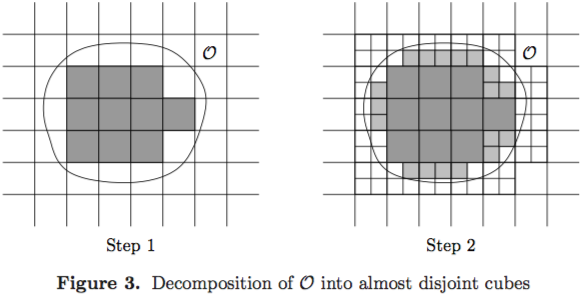
\includegraphics[scale=0.5]{fig3}
        \end{center}
        This procedure is then repeated indefinitely, and (by construction) the resulting collection $\mathcal{Q}$ of all accepted
        cubes is countable and consists of almost disjoint cubes. To see why their union is all of $O$, we note that
        given $x\in O$ there exists a cube of side length $2^{-N}$ that contains $x$ and that is entirely contained in $O$. Either
        this cube has been accepted, or it is contained in a cube that has been previously accepted. This shows that the union of
        all cubes in $\mathcal{Q}$ is $O$.
    \end{proof}

    \newpage

    \section{The exterior measure}
    
    In order to develop a suitable measure to work with in this course, we will first develop the Lebesgue \textit{outer} measure
    which can measure any set of $\mathbb{R}^d$ (by Vitali, this should not have one of the other properties of measure) and then
    restrict the size of the number of sets we can measure to obtain all the desired properties of a measure.\\

    \begin{definition}
        If $E$ is \textit{any} subset of $\mathbb{R}^d$, the \textbf{exterior} or \textbf{outer} measure of $E$ is defined as:
        \[ m_*(E) = \inf\sum_{j=1}^{\infty} |Q_j|,\]
        where the infimum is taken over all countable coverings $E\subset \cup_{j=1}^{\infty} Q_j$ by closed cubes. The exterior
        measure is always non-negative but could be infinite so, in particular, we have $m_*: \mathcal{P}(\mathbb{R}^d) \to [0,\infty]$.
    \end{definition}

    \begin{remark}
        The infimum always exists since it is bounded and taken over a non-empty set. Suppose for some $A$, $m_*(A) = 42$. This
        means:
        \begin{enumerate}
            \item For all countable coverings by closed cubes, $A\subset\cup_{j=1}^{\infty} Q_j$, so $\sum_{j=1}^{\infty} |Q_j|\geq 42$.
            \item For all $\epsilon>0$, there exists a countable covering: $A\subseteq\cup_{j=1}^{\infty} Q_j$ by closed cubes
                such that $\sum_{j=1}^{\infty} |Q_j| \leq 42 + \epsilon$.
        \end{enumerate}
        We can also replace the coverings by cubes with coverings by rectangles or even converings by balls.
    \end{remark}

    \begin{es}
        \begin{enumerate}
            \item $m_*(\emptyset) = 0$. This follows from the fact that any cube of arbitrary volume covers $\emptyset$.
            \item $m_*(\{x\in\mathbb{R}^d\}) = 0$. $x$ is covered by $[p-\nicefrac{1}{n},p+\nicefrac{1}{n}]$
                which are cubes of arbitrary length (by variying $n$).
            \item $m_*(\mathbb{Z}^+) = 0$ where $\mathbb{Z}^+$ are the positive integers. Given $\epsilon>0$, choose
                $Q_j = [j-\nicefrac{\epsilon}{2^{j+1}},j+\nicefrac{\epsilon}{2^{j+1}}]$. Then $\mathbb{Z}^+\subset\cup_{j=1}^{\infty}
                Q_j$ and
                \[ \sum_{j=1}^{\infty} |Q_j| = \sum_{j=0}^{\infty} \nicefrac{\epsilon}{2^j} = \epsilon \]
                so that $m_*(\mathbb{Z}^+) = 0$.
            \item Other examples of outer measure being zero include $\mathbb{Z},\mathbb{Z}^d,\mathbb{Q}$.
            \item Let $Q$ be a closed cube in $\mathbb{R}^d$. Simply cover it by itself to obtain $m_*(Q)\leq |Q|$. It is left
                to prove the reverse inequality. We consider an arbitrary cover $Q\subset\cup_{j=1}^{\infty} Q_j$ by cubes,
                and note that it suffices to prove that
                \[ |Q| \leq \sum_{j=1}^{\infty} |Q_j| \]
                Fix $\epsilon>0$. Choose for each $j$ and cube $S_j$ which contains $Q_j$, and such that $|S_j|\leq (1+\epsilon)|Q_j|$.
                From the open covering $\cup_{j=1}^{\infty} S_j$ of the compact set $Q$, we may select a finite subcovering which,
                after possibly renumbering the rectangles ,we may write as $Q\subset\cup_{j=1}^N S_j$. Taking the closure of the cubes
                $S_j$, we may apply Lemma 4 to conclude $|Q|\leq \sum_{j=1}^N |S_j|$. Consequently,
                \[ |Q| \leq (1+\epsilon)\sum_{j=1}^N |Q_j| \leq (1+\epsilon)\sum_{j=1}^{\infty} |Q_j| \]
                Since $\epsilon$ is aribtrary, we find that the inequality we wanted to prove holds; thus $|Q|\leq m_*(Q)$ as desired.
            \item If $Q$ is an open cube, the result $m_*(Q) = |Q|$ still holds. Since $Q$ is covered by its closure $|\overline{Q}|$,
                and $|\overline{Q}| = |Q|$, we immediately see that $m_*(Q) \leq |Q|$. Now, for the reverse inequality. Note that if
                $Q_0$ is a closed cube contained in $Q$, then $m_*(Q_0)\leq m_*(Q)$, since any covering of $Q$ by a countable number
                of closed cubes is also a covering of $Q_0$. Hence $|Q_0|\leq m_*(Q)$, and since we can choose $Q_0$ with a volume
                of as close as we wish to $|Q|$, we musth have $|Q|\leq m_*(Q)$.
            \item $m_*(\mathbb{R}^d) = \infty$
            \item $m_*(C) = 0$ where $C$ is the Cantor set
            \item $m_*(R) = |R|$ where $R$ is a rectangle.
        \end{enumerate}
    \end{es}

    \subsection{Properties of the exterior measure}

    Now, we cover some of the properties of this exterior measure.

    \begin{obs}[Monotonicity]
        If $A_1\subseteq A_2$, then $m_*(A_1)\leq m_*(A_2)$.
    \end{obs}
    \begin{proof}
        It suffices to note that any covering of $A_2$ covers $A_1$.
    \end{proof}

    \begin{obs}[Countable subadditivity]
        If $A=\cup_{j=1}^{\infty} A_j$, then $m_*(A) \leq \sum_{j=1}^{\infty} m_*(A_j)$.
    \end{obs}
    \begin{proof}
        Fix $\epsilon>0$. For each $j$, there is a countable covering $A_j\subset \cup_{j=1}^{\infty} Q_{j_k}$ by closed cubes
        such that
        \[ \sum_{j=1}^{\infty} |Q_{j_k}| \leq m_*(A_j) + \nicefrac{\epsilon}{2^j} \]
        Then $A\subset \cup_{j,k=1}^{\infty} Q_{j,k}$ is a countable covering by closed cubes and:
        \begin{align*}
            \sum_{j,k=1}^{\infty} |Q_{j,k}| &= \sum_{j=1}^{\infty} \sum_{k=1}^{\infty} |Q_{j,k}| \\
            &\leq \sum_{j=1}^{\infty} [m_*(A_j)+\nicefrac{\epsilon}{2^j}] \\
            &= \sum_{j=1}^{\infty} m_*(A_j) + \epsilon \\
            &= m_*(A) \leq \sum_{j=1}^{\infty} m_*(A_j) 
        \end{align*}
        where hte last equality follows from the fact that $\epsilon$ is arbitrary.
    \end{proof}

    \begin{obs}[Outer approximation]
        $m_*(A) = \inf_{A\subset O\:\text{open}} m_*(A)$.
    \end{obs}
    \begin{proof}
        $A\subset O$ open implies $m_*(A) \leq m_*(O)$ which the implies $m_*(A) \leq \inf_{A\subset O\:\text{open}} m_*(O)$.
        To show the other inequality, we have to show $\inf_{A\subset O\:\text{open}} m_*(O) \leq m_*(A)$ i.e.
        \[ \forall\;\epsilon>0,\;\exists\;A\subset O\;\text{open},\;\text{such that}\; m_*(O) \leq m_*(A) + \epsilon \]
    \end{proof}

\end{document}
